\documentclass{beamer}
\usepackage[utf8]{inputenc}

\usetheme{Madrid}
\usecolortheme{default}
\usepackage{amsmath,amssymb,amsfonts,amsthm}
\usepackage{txfonts}
\usepackage{tkz-euclide}
\usepackage{listings}
\usepackage{adjustbox}
\usepackage{array}
\usepackage{tabularx}
\usepackage{gvv}
\usepackage{lmodern}
\usepackage{circuitikz}
\usepackage{tikz}
\usepackage{graphicx}

\setbeamertemplate{page number in head/foot}[totalframenumber]

\usepackage{tcolorbox}
\tcbuselibrary{minted,breakable,xparse,skins}



\definecolor{bg}{gray}{0.95}
\DeclareTCBListing{mintedbox}{O{}m!O{}}{%
  breakable=true,
  listing engine=minted,
  listing only,
  minted language=#2,
  minted style=default,
  minted options={%
    linenos,
    gobble=0,
    breaklines=true,
    breakafter=,,
    fontsize=\small,
    numbersep=8pt,
    #1},
  boxsep=0pt,
  left skip=0pt,
  right skip=0pt,
  left=25pt,
  right=0pt,
  top=3pt,
  bottom=3pt,
  arc=5pt,
  leftrule=0pt,
  rightrule=0pt,
  bottomrule=2pt,
  toprule=2pt,
  colback=bg,
  colframe=orange!70,
  enhanced,
  overlay={%
    \begin{tcbclipinterior}
    \fill[orange!20!white] (frame.south west) rectangle ([xshift=20pt]frame.north west);
    \end{tcbclipinterior}},
  #3,
}
\lstset{
    language=C,
    basicstyle=\ttfamily\small,
    keywordstyle=\color{blue},
    stringstyle=\color{orange},
    commentstyle=\color{green!60!black},
    numbers=left,
    numberstyle=\tiny\color{gray},
    breaklines=true,
    showstringspaces=false,
}
%------------------------------------------------------------
%This block of code defines the information to appear in the
%Title page
\title %optional
{4.7.13}
\date{13 September, 2025}
%\subtitle{A short story}

\author % (optional)
{INDHIRESH S - EE25BTECH11027}



\begin{document}


\frame{\titlepage}
\begin{frame}{Question}
 Find the distance between the lines $l_1$ and $l_2$ given by
\begin{align*}
    \overrightarrow{r}=\hat{i}+2\hat{j}-4\hat{k}+\lambda(2\hat{i}+3\hat{j}+6\hat{k})\\\overrightarrow{r}=3\hat{i}+3\hat{j}-5\hat{k}+\mu(2\hat{i}+3\hat{j}+6\hat{k})
\end{align*}
\end{frame}
\begin{frame}{allowframebreaks}
\frametitle{Equation}

    \centering
    
    \label{tab:parameters}
Given equation:
\begin{align}
   \Vec{r}=\hat{i}+2\hat{j}-4\hat{k}+\lambda(2\hat{i}+3\hat{j}+6\hat{k}) \\
\Vec{r}=3\hat{i}+3\hat{j}-5\hat{k}+\mu(2\hat{i}+3\hat{j}+6\hat{k})\\
\end{align}

   
\end{frame}


\begin{frame}
\frametitle{Theoretical Solution}
From the above two equation it is clear that given two lines are parallel.\\
Now we'll find the distance between them.\\
The given lines are in the form:
\begin{align}
   \Vec{r} = \myvec{1\\2\\-4} + k_1\myvec{2\\3\\6}\\
   \Vec{r} = \myvec{3\\3\\-5}+ k_2\myvec{2\\3\\6}
\end{align}
Where,
\begin{align}
    \Vec{A}=\myvec{1\\2\\-4}\;\;\,\Vec{B}=\myvec{3\\3\\-5}\;\;,\Vec{M}=\myvec{2&2\\3&3\\6&6}
\end{align}


\end{frame}
\begin{frame}
\frametitle{Theoretical solution}
From Least squares solution, for shortest distance:
\begin{align}
    \Vec{M^T}\Vec{M}\myvec{k_1\\-k_2}=\Vec{M^T}(\Vec{B}-\Vec{A})
\end{align}
\begin{align}
    \myvec{2&3&6\\2&3&6}\myvec{2&2\\3&3\\6&6}\myvec{k_1\\-k_2}=\myvec{2&3&6\\2&3&6}\brak{\myvec{3\\3\\-5}-\myvec{1\\2\\-4}}
\end{align}
\begin{align}
\myvec{49&49\\49&49}\myvec{k_1\\-k_2}=\myvec{2&3&6\\2&3&6}\brak{\myvec{3\\3\\-5}-\myvec{1\\2\\-4}}
\end{align}
\begin{align}
    \myvec{49&49\\49&49}\myvec{k_1\\-k_2}=\myvec{2&3&6\\2&3&6}\myvec{2\\1\\-1}
\end{align}






\end{frame}
\begin{frame}
\frametitle{Theoretical Solution}
    \begin{align}
   \myvec{49&49\\49&49}\myvec{k_1\\-k_2}=\myvec{1\\1}
\end{align}
\begin{align}
   \myvec{1&1\\1&1}\myvec{k_1\\-k_2}=\frac{\myvec{1\\1}}{49}
\end{align}
\begin{align}
     k_1-k_2=\frac{1}{49}
\end{align}
Let $r_1$ and $r_2$ be the point on the line $l_1$ and $l_2$\\
Now,
\begin{align}
    r_1-r_2=\myvec{-2\\-1\\1}+(k_1-k_2)\myvec{2\\3\\6}
\end{align}



\end{frame}
\begin{frame}
\frametitle{Theoretical Solution}
  \begin{align}
      r_1-r_2=\myvec{-2\\-1\\1}+(\frac{1}{49})\myvec{2\\3\\6}
\end{align}
\begin{align}
       r_1-r_2=\myvec{\frac{-96}{49}\\\\\frac{-46}{49}\\\\\frac{55}{49}}
\end{align}




\end{frame}

\begin{frame}
\frametitle{Theoretical Solution}
 Now , Distance between two lines = $\norm{r_1-r_2}$
\begin{align}
    \norm{r_1-r_2}=\sqrt{\brak{\frac{-96}{49}}^2+\brak{\frac{-46}{49}}^2+\brak{\frac{55}{49}}^2}
\end{align}
\begin{align}
       \norm{r_1-r_2}=\frac{\sqrt{14357}}{49}
\end{align}


Therefore the distance between the lines $l_1$ and $l_2$ is $\frac{\sqrt{14357}}{49}$

\end{frame}






\begin{frame}[fragile]
    \frametitle{C Code  }

    \begin{lstlisting}
#include <stdio.h>
#include <math.h>

int main() {
    double A[3] = {1,2,-4};
    double B[3] = {3,3,-5};
    double d[3] = {2,3,6};
    double AB[3], cross[3];
    double dist;

    // Compute B - A
    for(int i=0;i<3;i++) AB[i] = B[i] - A[i];

    // Cross product (AB x d)
    cross[0] = AB[1]*d[2] - AB[2]*d[1];
    cross[1] = AB[2]*d[0] - AB[0]*d[2];
    cross[2] = AB[0]*d[1] - AB[1]*d[0];

    


    \end{lstlisting}
\end{frame}

\begin{frame}[fragile]
    \frametitle{C Code  }

    \begin{lstlisting}


    // Norms
    double num = sqrt(cross[0]*cross[0] + cross[1]*cross[1] + cross[2]*cross[2]);
    double den = sqrt(d[0]*d[0] + d[1]*d[1] + d[2]*d[2]);

    dist = num / den;
    printf("Distance between lines = %lf\n", dist);

    // Output A, B, direction vector for plotting
    printf("A: %lf %lf %lf\n", A[0], A[1], A[2]);
    printf("B: %lf %lf %lf\n", B[0], B[1], B[2]);
    printf("d: %lf %lf %lf\n", d[0], d[1], d[2]);

    return 0;
}


    \end{lstlisting}
\end{frame}


\begin{frame}[fragile]
    \frametitle{Python Code}
    \begin{lstlisting}
import ctypes
import numpy as np
import matplotlib.pyplot as plt
from mpl_toolkits.mplot3d.art3d import Poly3DCollection

# Load shared C library
lib = ctypes.CDLL("./distance.so")
lib.main()

# Define points and direction vector (same as in C)
A = np.array([1,2,-4])
B = np.array([3,3,-5])
d = np.array([2,3,6])

# Generate points for both lines
t = np.linspace(-2,2,10)
line1 = A[:,None] + d[:,None]*t
line2 = B[:,None] + d[:,None]*t












    \end{lstlisting}
\end{frame}

\begin{frame}[fragile]
    \frametitle{Python Code}
    \begin{lstlisting}
# Plot
fig = plt.figure()
ax = fig.add_subplot(111, projection='3d')

# Lines
ax.plot(line1[0], line1[1], line1[2], 'b-', label='Line l1')
ax.plot(line2[0], line2[1], line2[2], 'g-', label='Line l2')

# Points
ax.scatter(*A,color='r',s=50)
ax.text(*A,"A(1,2,-4)",color='red')
ax.scatter(*B,color='orange',s=50)
ax.text(*B,"B(3,3,-5)",color='orange')

# Dotted line AB
ax.plot([A[0],B[0]], [A[1],B[1]], [A[2],B[2]], 'k--', label='Connecting AB')













    \end{lstlisting}
\end{frame}

\begin{frame}[fragile]
    \frametitle{Python Code}

    \begin{lstlisting}
ax.set_title("Figure")
ax.set_xlabel("X-axis")
ax.set_ylabel("Y-axis")
ax.set_zlabel("Z-axis")
ax.legend()
plt.savefig("/media/indhiresh-s/New Volume/Matrix/ee1030-2025/ee25btech11027/MATGEO/4.7.13/figs/figure1.png")
plt.show()






    \end{lstlisting}
\end{frame}



\begin{frame}{Plot}
    \begin{center}
        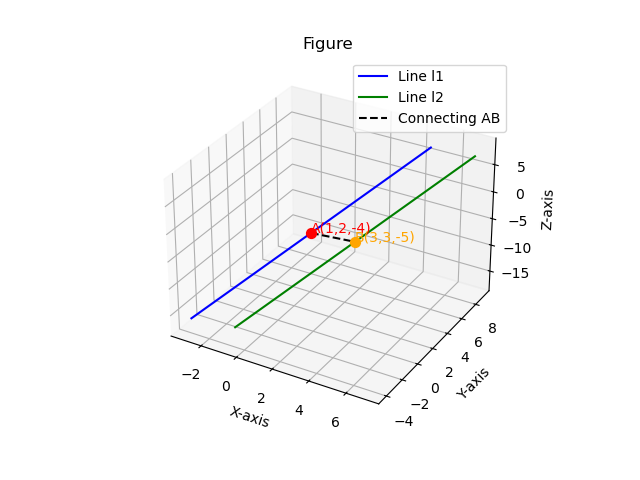
\includegraphics[width=\columnwidth, height=0.8\textheight, keepaspectratio]{figs/figure1.png}
    \end{center}
\end{frame}




\end{document}